
\subsection{Trigger Performance}

As described above, the primary physics trigger is based on the total
energy observed in the calorimeter, combined with a requirement of a
single incoming electron observed in the trigger fiber hodoscope.
Figure~\ref{fig:trigger_rejection} shows the simulated performance of
the primary physics trigger for signal and background.

\begin{figure}[t]
  \begin{center}
    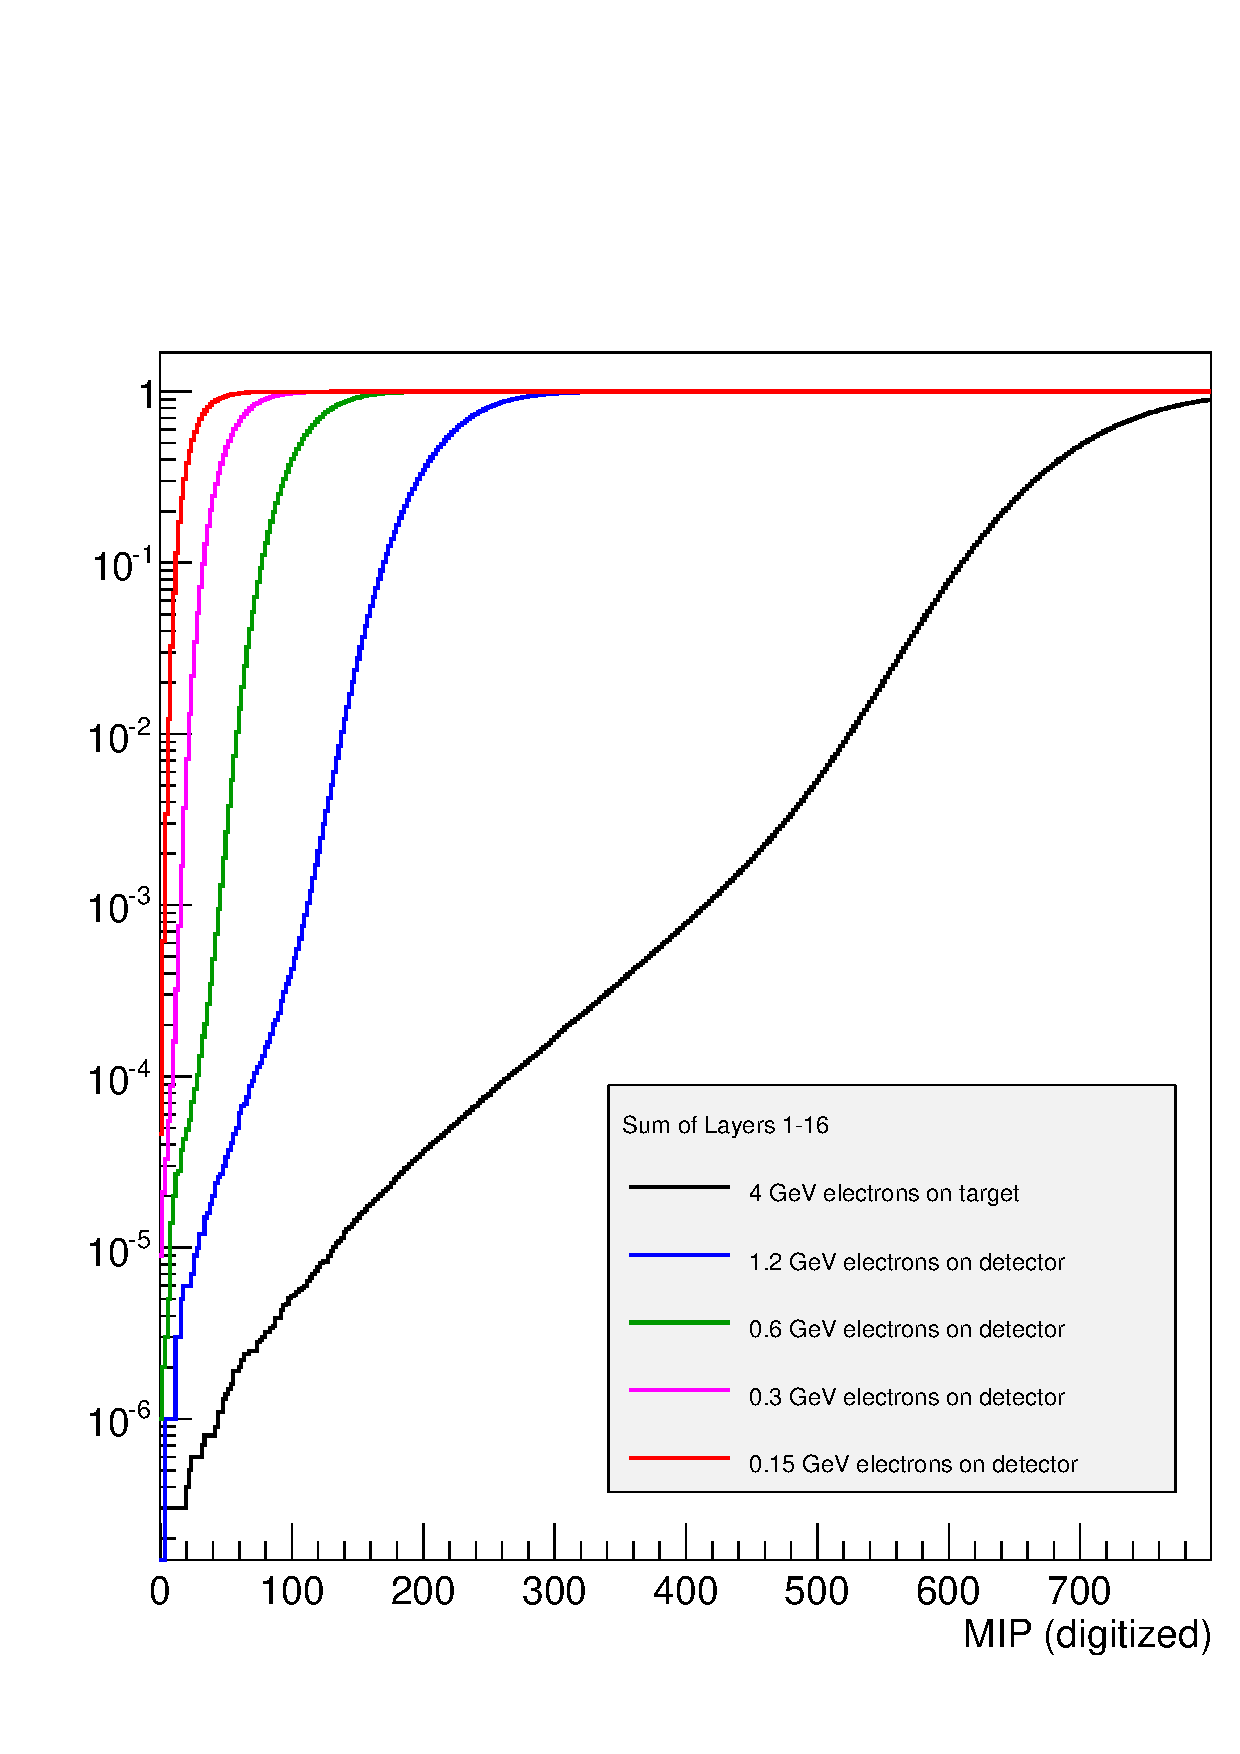
\includegraphics[width=0.7\linewidth]{images/trigger/trigger_rates_energy}
    \end{center}
  \caption{Performance of the primary physics trigger for LDMX.  The
    effiency for signal electrons of differing energy and the trigger
    rate for all backgrounds induced by beam electrons are shown as a
    function of the trigger threshold in MIP
    units.}\label{fig:trigger_rejection}
\end{figure}

Besides the primary physics trigger, the LDMX trigger system will also
allow the selection of events for calibration, alignment, and
background studies.  The trigger will include input from the
scintillator calorimeter to allow selection of events with hadrons or
muons.  Each event will be marked with the set of triggers which
fired.  An initial draft trigger menu is shown in Table~\ref{tab:trigger_menu}.

\begin{table}
  \caption{Draft trigger menu for LDMX, showing the primary
    contributions to the trigger budget for a 46~MHz beam
    rate}\label{tab:trigger_menu}
  \begin{tabular}{|l|r|r|} \hline
    Trigger & Prescale factor & Rate (Hz) \\
    \hline
    \em{Physics Trigger} & 1 & \\ 
    \hspace{0.2in} $\mathrm{E(ECAL)}<1.2$~GeV & & 4600 \\ \hline
    \em{Background-Measurement Triggers} &  & \em{100} \\
    \hspace{0.2in} $\mathrm{E(ECAL)}>3$~GeV & & 25 \\
    \hspace{0.2in} $\mathrm{E(ECAL)}>2$~GeV & & 50 \\
    \hspace{0.2in} HCAL single MIP trigger & & 25 \\ \hline
    \em{Detector-Monitoring Triggers} &  & \em{50} \\
    \hspace{0.2in} Beam-arrival (hodoscope) & 4000000 & 10 \\
    \hspace{0.2in} Empty-detector (hodoscope veto) & & 10 \\
    \hline
  \end{tabular}
  \\
  \draft{Allocations are extremely rough at the moment!}
\end{table}


\begin{enumerate}
\item What is the rate of muon production?  We would expect to trigger these, yes?
\item What is the impact of cosmics on the HCAL trigger?
\end{enumerate}
